\section{Multi-Robot Systems}

\begin{frame}
	\frametitle{Approaches to evaluate Multi-Robot Systems}
	
	Can be divided in 4 categories
	\vspace{0.2cm}
	
	\begin{itemize}
		\large
		\item \textbf{simulated robots + perfect network (centralized process)}
		
		\begin{itemize}
			\small \item e.g. Stage + everything running on a single machine
		\end{itemize}
		
		\vspace{0.05cm}
		\item \textbf{simulated robots + perfect network (distributed process)}
		
		\begin{itemize}
			\small \item e.g. Stage + each robot runs on a different machine
		\end{itemize}
		
		\vspace{0.05cm}
		\item \textbf{simulated robots + simulated network}
		
		\begin{itemize}
			\small \item e.g. Stage + ns-3
		\end{itemize}
		
		\vspace{0.05cm}
		\item \textbf{real robots}
	\end{itemize}
\end{frame}

\begin{frame}
	\frametitle{Preliminary Results in Tracking Mobile Targets Using Range Sensors from Multiple Robots}
	
	\normalsize
	
	\vspace{0.3cm}
	
	\begin{block}{Goal}
		tracking humans while they are within range of the robot team sensors
	\end{block}
	
	\vspace{0.15cm}
	
	\textbf{Parameters evaluated}
	
	\begin{itemize}
		\item Humans' estimation accuracy
	\end{itemize}
	
	\textbf{Platform}
	
	\begin{itemize}
		\item Player/Stage
	\end{itemize}
	
	\textbf{Category}
	
	\begin{itemize}
		\item simulated robots + perfect network (centralized process)
	\end{itemize}
	
	\vspace{-4cm}
	
	\begin{tabbing}
		\hspace{7cm}
		
		\begin{tikzpicture}
			\node at (0,0) [draw=black,ultra thick,inner sep=0pt]  {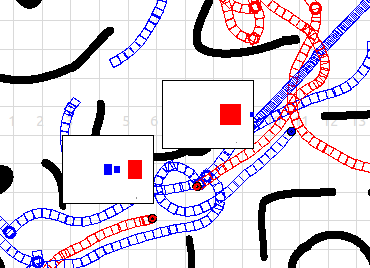
\includegraphics[width=3.5cm]{Images/Stage.png}};
		\end{tikzpicture}
	\end{tabbing}
	
	\vspace{0.9cm}
	
	\tiny
	E. Liao at al, \emph{Preliminary Results in Tracking Mobile Targets Using Range Sensors from Multiple Robots},
	\vspace{-0.35cm}
	Distributed Autonomous Robotic Systems, 2006.
\end{frame}

\begin{frame}
	\frametitle{Preliminary Results in Tracking Mobile Targets Using Range Sensors from Multiple Robots}
	
	\textbf{Assumptions}
	
	\begin{itemize}
		\item Explicit
		
		\begin{itemize}
			\item robots are always localized
		\end{itemize}
		
		\item Implicit
		
		\begin{itemize}
			\item no communication delay
			
			\item no messages lost
		\end{itemize}
	\end{itemize}
\end{frame}

\begin{frame}
	\frametitle{Preliminary Results in Tracking Mobile Targets Using Range Sensors from Multiple Robots}
	
	\textbf{Experiment:} Four robots move around the map using a coordination strategy, attempting to localize the
	firefighters using simulated ranging measurements. Different levels of artificial noise have been added
\end{frame}

\begin{frame}
	\frametitle{Preliminary Results in Tracking Mobile Targets Using Range Sensors from Multiple Robots}
	\framesubtitle{System evaluation}
	
	\begin{itemize}
		\item \textbf{Humans' estimation accuracy:} averaged euclidean distance between actual and observed humans
			  over all the runs performed
	\end{itemize}
\end{frame}

\begin{frame}
	\frametitle{Comments}
	
	\textbf{Open questions}
	
	\begin{enumerate}
		\item \emph{What could be the impact of a communication delay?}
		
		\item \emph{What guarantees the same performance in a real scenario?}
	\end{enumerate}
\end{frame}

\begin{frame}
	\frametitle{Coordination in a Multi-Robot Surveillance Application using Wireless Sensor Networks}
	
	\normalsize
	
	\vspace{0.3cm}
	
	\begin{block}{Goal}
		investigate the problem of multi-robot coordination for target tracking and capturing
	\end{block}
	
	\vspace{0.15cm}
	
	\begin{columns}[T]
		\column{0.5\textwidth}
		
		\textbf{Parameters evaluated}
		
		\begin{itemize}
			\item Robot traveled distance
			
			\item Mission time
		\end{itemize}
		
		\column{0.5\textwidth}
		
		\textbf{Platform}
		
		\begin{itemize}
			\item Player/Stage
		\end{itemize}
	\end{columns}
	
	\vspace{0.5cm}
	
	\textbf{Category}
	
	\begin{itemize}
		\item simulated robots + perfect network (distributed processes)
	\end{itemize}
	
	\tiny
	S. Trigui at al, \emph{Coordination in a Multi-Robot Surveillance Application using Wireless Sensor Networks},
	\vspace{-0.35cm}
	16th IEEE Mediterranean, 2012.
\end{frame}

\begin{frame}
	\frametitle{Coordination in a Multi-Robot Surveillance Application using Wireless Sensor Networks}
	
	\textbf{Assumptions}
	
	\begin{itemize}
		\item no communication overhead
		
		\item no communication delay
		
		\item no complete knowledge of the environment
	\end{itemize}
\end{frame}

\begin{frame}
	\frametitle{Coordination in a Multi-Robot Surveillance Application using Wireless Sensor Networks}
	
	\textbf{Experiment 1:} the number of pursuers is greater than the number of intruders
	
	\vspace{0.4cm}
	
	\textbf{Experiment 2:} the number of pursuers is smaller than the number of intruders
	
	\vspace{0.4cm}
	
	\textbf{Experiment 3:} the number of pursuers is equal to the number of intruders
\end{frame}

\begin{frame}
	\frametitle{Coordination in a Multi-Robot Surveillance Application using Wireless Sensor Networks}
	\framesubtitle{System evaluation}
	
	\begin{itemize}
		\item \textbf{Robot traveled distance:} in each experiment is averaged over the number of pursuers
		
		\vspace{0.3cm}
		
		\item \textbf{Mission time:} the time needed to complete the mission (averaged over 30 runs)
	\end{itemize}
\end{frame}

\begin{frame}
	\frametitle{Comments}
	
	\textbf{Open questions}
	
	\begin{enumerate}
		\item \emph{What could be the impact of a communication delay?}
		
		\item \emph{How could a real network affect the system performance?}
	\end{enumerate}
\end{frame}

\begin{frame}
	\frametitle{Distributed Sensor Fusion for Object Position Estimation by Multi-Robot Systems}
	
	\normalsize
	
	\vspace{0.3cm}
	
	\begin{block}{Goal}
		estimations of the location of dynamic objects that are simultaneously visible by multiple robots
	\end{block}
	
	\vspace{0.15cm}
	
	\textbf{Parameters evaluated}
	
	\begin{itemize}
		\item Distributed Data Fusion
		
		\item Object estimation accuracy
	\end{itemize}
	
	\textbf{Platform}
	
	\begin{itemize}
		\item Cye robot
	\end{itemize}
	
	\vspace{-3.7cm}
	
	\begin{tabbing}
		\hspace{7cm}
		
		\begin{tikzpicture}
			\node at (0,0) [draw=black,ultra thick,inner sep=0pt]  {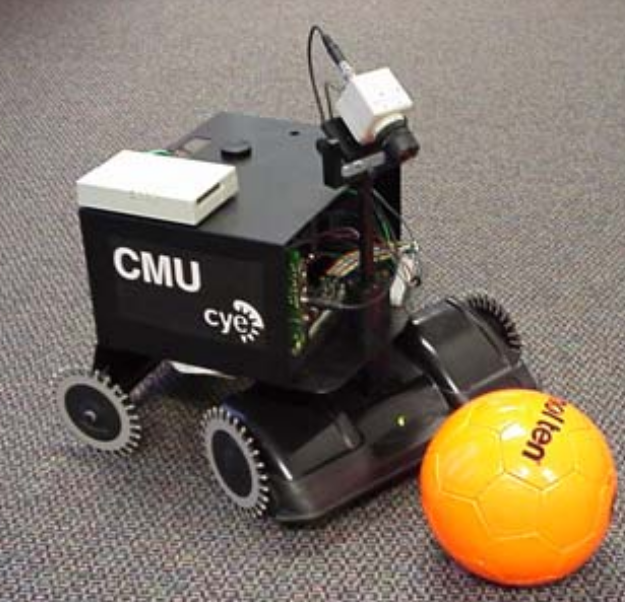
\includegraphics[width=3.5cm]{Images/CyeRobot.png}};
		\end{tikzpicture}
	\end{tabbing}
	
	\vspace{-0.5cm}
	
	\tiny
	W. Stroupe at al, \emph{Distributed Sensor Fusion for Object Position Estimation by Multi-Robot Systems},
	\vspace{-0.35cm}
	Proceedings 2001 ICRA. IEEE International Conference on Robotics and Automation.
\end{frame}

\begin{frame}
	\frametitle{Distributed Sensor Fusion for Object Position Estimation by Multi-Robot Systems}
	
	\textbf{Assumptions}
	
	\begin{itemize}
		\item sensor errors are independent
		
		\item robot is perfectly localized
		
		\item high frame rates
		
		\item low object speeds
	\end{itemize}
\end{frame}

\begin{frame}
	\frametitle{Distributed Sensor Fusion for Object Position Estimation by Multi-Robot Systems}
	
	\textbf{Experiment 1:} three Cye robots tracking a ball in fixed discrete positions in the environment
	
	\vspace{0.4cm}
	
	\textbf{Experiment 2:} a Cye robot sees an object that is unreachable for him, so another robot that cannot
	see the object, reaches it using the observations provided by the first one
	
	\vspace{0.4cm}
	
	\textbf{Experiment 3:} RoboCup middle-size where robots sharing the information of the ball
\end{frame}

\begin{frame}
	\frametitle{Distributed Sensor Fusion for Object Position Estimation by Multi-Robot Systems}
	
	\vspace{0.7cm}
	
	\textbf{Preconditions}
	
	\begin{itemize}
		\item built a model of the sensors' error
	\end{itemize}
	
	\vspace{0.2cm}
	
	\textbf{Evaluation}
	
	\begin{enumerate}
		\item ball location measured by each robot was recorded
		
		\item these individual observations were merged together and in pairs
		
		\item \textbf{euclidean distance} between actual and observed object
	\end{enumerate}
\end{frame}

\begin{frame}
	\frametitle{Comments}
	
	\textbf{Open questions}
	
	\begin{enumerate}
		\item \emph{How does the position precision change based on the localization accuracy?}
	\end{enumerate}
\end{frame}

\begin{frame}
	\frametitle{A Framework for Realistic Simulation of Networked Multi-Robot Systems}
	
	\normalsize
	
	\vspace{0.3cm}
	
	\begin{block}{Goal}
		a communication-realistic simulation tool to help understanding the relation between the quality of
		communication and the operation of a large-scale cooperative multi-robot system
	\end{block}
	
	\vspace{0.15cm}
	
	\begin{columns}[T]
		\column{0.5\textwidth}
		
		\textbf{Parameters evaluated}
		
		\begin{itemize}
			\item Computational performance
			
			\item Generated overhead
		\end{itemize}
		
		\column{0.5\textwidth}
		
		\textbf{Platform}
		
		\begin{itemize}
			\item Combining simulators
			
			\begin{itemize}
				\item ARGoS
				
				\item ns-3
			\end{itemize}
		\end{itemize}
	\end{columns}
	
	\textbf{Category}
	
	\begin{itemize}
		\item simulated robots + simulated network
	\end{itemize}
	
	\vspace{-0.12cm}
	
	\tiny
	M. Kudelski at al, \emph{A Framework for Realistic Simulation of Networked Multi-Robot Systems},
	\vspace{-0.35cm}
	2012 IEEE/RSJ International Conference on Intelligent Robots and Systems.
\end{frame}

\begin{frame}
	\frametitle{A Framework for Realistic Simulation of Networked Multi-Robot Systems}
	
	\textbf{Assumptions}
	
	\begin{itemize}
		\item simulation time needs to be synchronized
		
		\item system's state must be efficiently exchanged between simulators
	\end{itemize}
\end{frame}

\begin{frame}
	\frametitle{A Framework for Realistic Simulation of Networked Multi-Robot Systems}
	
	\textbf{Experiment:} use the integrated ARGoS/ns-3 environment in a scenario to study the distributed
	coordination of robots cooperatively performing task assignment
\end{frame}

\begin{frame}
	\frametitle{A Framework for Realistic Simulation of Networked Multi-Robot Systems}
	\framesubtitle{System evaluation}
	
	\begin{itemize}
		\item \textbf{Computational performance:} CPU time consumed is measured varying the number of simulated
			  robots between 25 and 250 and 20\% of nodes generate network traffic
		
		\vspace{0.3cm}
		
		\item \textbf{Overhead:} difference between the CPU time consumed by the combined simulators and the CPU time
			  consumed by the standalone ARGoS with the simplified communication model
	\end{itemize}
\end{frame}
